\documentclass{article}
\title{Mean Shift Summary}
\author{Shuo Sun}
\date{07/09/2021}
\usepackage{amsmath}
\usepackage{graphicx}
\usepackage{subfigure}
\usepackage[labelfont=it, textfont={bf,it}, font=small ]{caption}
\usepackage{subcaption}
\usepackage[ruled]{algorithm2e}
\begin{document}

\maketitle

\section{Introduction}
\paragraph{
The MS(Mean Shift) algorithm is a kind of clustering algorithm based on density estimation.Given discretely sampled data, the MS algorithm aims to locate the maxima of the density function. To estimate the density function, one simple approach is to smooth the data, for example:
}
\begin{equation}
f(x) = \sum_{i=1}^{N}K(\frac{x-x_i}{h})
\end{equation}
\subparagraph{
——The function K(x) is called the *kernel function* if there exists a profile such that:
}
\begin{equation}
K(x) = k(||x||^2)
\end{equation}

\subparagraph{
the $k(x)$ should have the property:\\
1) $k$ in non-negative\\
2) $k$ is non-increasing: $k(a) \geq k(b)$ if $a < b$\\
3) $k$ is piecewise continuous and $\int_{0}^{\infty}k(r)d(r) < \infty $
}

\subparagraph{
The sample mean with kernel K at $x \in X$ can be written as :
}

\begin{equation}
m(x) = \frac{\sum_{s\in S'}K(s-x)w(s)s}{\sum_{s \in S'}K(s-x)w(s)}
\end{equation}

\subparagraph{
——where $S'$ is the a finite set(sample); $w(s)$ is the weight function.
}

\subparagraph{
Let $T \subset  X$ is a finite set, and we use the MS algorithm iteratively  $T \leftarrow m(T)$ until converging.  If the set $T = S$, we call it a blurring process.
}
\subparagraph{
Based on the above information, we can simply summarise the process of the Mean Shift algorithm:
}
%%%
%\begin{algorithm}
%\caption{Mean Shift}
%\KwData{sample set: $S'$, point set: $T$, bandwidth: $h$, threshold: $\epsilon$}
%\KwResult{shifting\_points set: $T'$}
%\end{algorithm}
%%%

\subparagraph{
In this task, I give two different ways for Mean-Shift algorithm to process circular-linear data. The difference of two ways is how to compute the evaluate the distance between two point with $(\theta, r)$ format. The first one (Algo1) converts the point in polar coordinate to Cartesian coordinate. The second one (Algo2) directly computes the distance between two points like Euclidean space.
}

%---------------------------------- section 2 ------------------------------------------------%
\section{Methods}

\subsection{Distance between points}
\paragraph{
When we use the kernel function to estimate the density around the point $x$:
}
\begin{equation}
f(x) = \sum_{i=1}^{N}K(\frac{x-x_i}{h})
\end{equation}
\subparagraph{
In the above equation, $(x-x_i)$ is used to describe the \textit{distance} between points. Different ways of evaluating the distance can result in different density function. So the first thing to do is how to evaluate the distance between two points of circular-linear data.
}

\subsubsection{Algo1}
\paragraph{
The data given is a circular-linear data, with the format$(\theta, r)$. The variable $\theta$ represents direction, and the variable $r$ represents the size in the direction. It is an inituitive idea that we can convert the a vector in polar coordinate to a point in Cartesian coordinate:
}

\begin{equation}
\begin{aligned}
x = r \cos{\theta} \\
y = r \sin {\theta}
\end{aligned}
\end{equation}

\subparagraph{
We are familiar with the distance between two points in Cartesian coordinate:
}

\begin{equation}
d(p_{1}, p_{2}) = \sqrt{(x_{1} - x_{2})^2 + ({y_1 - y_2})^2}
\end{equation}

\subparagraph{
After getting the data with the format of $(\theta,r)$, the data should be pre-processed first. The set after processed is called $S_p$. In the successive steps, the data set $S_p$ will be used to find clusters.
}

\subsubsection{Algo2}
\paragraph{
We can also compute the distance directly on the raw data in a way similar to Cartesian coordinate:
}

\begin{equation}
d(p_1, p_2) = \sqrt{({\theta_1 - \theta_2})^2 + ({r_1 - r_2})^2}
\end{equation}

\subparagraph{
However, the variable $\theta$ is angle in $[0, 2 \pi]$, the angle is a kind of periodic value. That means the real distance between $0$ and $2\pi$ is $0$ , not $2\pi$. Similarly, the distance between $0$ and $\frac{3}{2} \pi$ is $\frac{1}{2} \pi$. As shown below:
}
\subparagraph{
\begin{figure}[h]
\centering
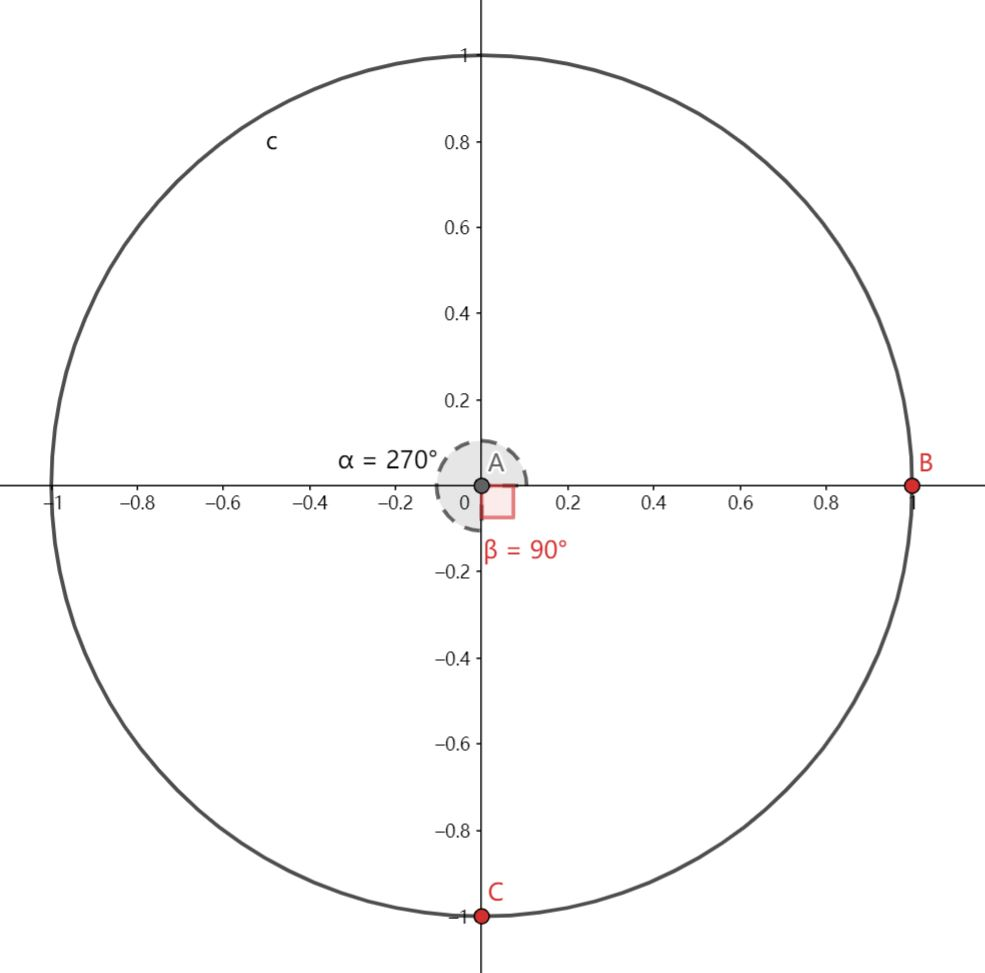
\includegraphics[width=7cm]{0-23}
\caption{Point B represents $0$, point C represents $3\pi/2$, the real \textit{distance} between B and C is {$\pi$}/{2}}
\end{figure}
}

\subparagraph{
    So, the distance between two angle should be:
}

\begin{equation}
    d(\theta_1, \theta_2) =
    \begin{cases}
    2\pi - |\theta_1 - \theta_2| &|\theta_1 - \theta_2|>\pi\\
    |\theta_1 - \theta_2|  &else
    \end{cases}
\end{equation}

\subparagraph{
    The distance of the circular-linear data is:
}

\begin{equation}
    d(v_1,v_2) = \sqrt{d^2(\theta_1 - \theta_2) + (r_1 - r_2)^2}
\end{equation}

% -------------------The section 2-------------------%
\subsection{Parameters choosing}
\subsubsection{Bandwidth}
\paragraph{
    The main parameter of the Mean Shift algorithm is the \textit{bandwidth} of kernel function.
    If h is small, the point with larger distance will have smaller weight. The fewer points will be used to estimate density, the variance will be larger. However, if h is large, this will result in bigger bias.
    So, there is a trade-off between bias and variance when choosing bandwidth. Given the size of sampled data N, the bandwidth should meet the requirement that $N\rightarrow \infty$, $h \rightarrow 0$. By this, we can get h should be :
}

\begin{equation}
    h = cN^{-1/5}
\end{equation}
\subparagraph{
    ——Where c is a constant.
}
\subparagraph{
    For the Guassian distributation, $h$ should be:
}

\begin{equation}
\begin{aligned}
    h &= (\frac{4\sigma^5}{3N})^{1/5}
&=\frac{1.05 * \sigma}{N^5}
\end{aligned}
\end{equation}
\subparagraph{——where $\sigma$ is the standard deviation for  the sample.}

\subsubsection{Kernel Function}
\paragraph{
    The common kernel function used is \textit{flat kernel} :
}

\begin{equation}
    F(x) =
    \begin{cases}
        1 &if ||x|| \le h\\
        0 &if ||x|| > h
        \end{cases}
\end{equation}
\subparagraph{and \textit{Gaussian kernel}:}

\begin{equation}
    G(x) = \frac{1}{h\sqrt{2\pi}} e^{-\frac{||x||^2}{2h^2}}
\end{equation}

\subparagraph{
    The kernel function can be seen as the weight to estimate the point around $x$.
    The \textit{flat kernel} can be seen as a d-dimensional sphere, only the point in this sphere will be considered.
    The \textit{Gaussian kernel} consider all the points in the set, but the closer point will have larger point.
}
\subparagraph{
    In this task, we will use the \textit{Gaussian kernel} as the kernel function.
}

\subsubsection{Weight Function}
\paragraph{
    Weight function $w(s)$ can be fixed or re-evaluated after each iteration. In this task, the Gaussian kenrl has already
    set the weight for each point, so I just set $w(s) = 1$ in the iteration.
}

\subsubsection{Threshold}
\paragraph{
    The parameter threshold is used to decide when to stop iteration. The larger threshold will result in more clusters. But smaller threshold may result in
    that thres is only one mode in the set. In this task, we will set different threshold and analyse the results.
}

%-------------------------section 3----------------------------%
\section{Data Analysis}
%----------section 3.1
\subsection{Computing Means}
\paragraph{
    After the iteration of Mean Shift algorithm, we can get different modes of data. To estimate the basic parameters of different modes,
    we need to find the centroid of each cluster by computing the mean point of each cluster.
}
\subparagraph{
    The simplest idea is $\bar{x} = \frac{1}{N} \sum_{i}^N{x_i}$. For $\theta$, it can be seen as a point on a unit circle. We can cut the circle and make it a line:
}

\subparagraph{
    \begin{figure*}[tp]
        \centering
        \subfigure[1]{
            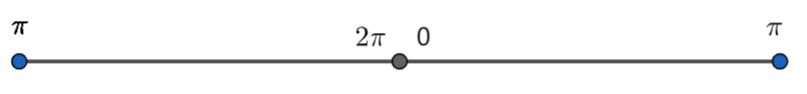
\includegraphics[width=\textwidth]{line2.JPG}
        }
        \subfigure[2]{
            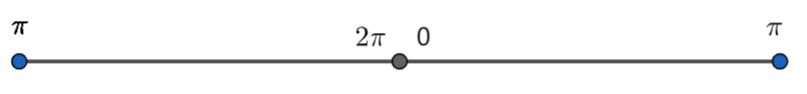
\includegraphics[width=\textwidth]{line2.JPG}
        }
    \end{figure*}
}

%----------section 3.2
\subsection{Computing Variance}
\end{document}